\documentclass[12pt,a4paper]{article}
\usepackage[UTF8]{ctex}
\usepackage{amsmath,amssymb}
\usepackage{xcolor}
\usepackage{hyperref}
\usepackage{geometry}
\usepackage{graphicx}
\geometry{margin=2.5cm}

\title{Lattice Shortest Vector Problem / 格最短向量问题}
\author{QuoNic}
\date{}

\begin{document}
\maketitle

\begin{center}
\textbf{Algorithms / 算法} | 难度：高级 | 预计时间：25 分钟
\end{center}

\tableofcontents
\newpage

\section{为什么需要？}

格最短向量问题是格密码学的基础，量子算法可以高效求解。

\subsection{经典局限}
\begin{itemize}
  \item 经典算法需要指数时间求解 SVP
  \item 对于高维格，经典方法效率低
\end{itemize}

\subsection{量子优势}
\begin{itemize}
  \item 量子算法可以在多项式时间内求解近似 SVP
  \item 提供指数加速
  \item 是后量子密码学的基础
\end{itemize}

\subsection{实际应用}
\begin{itemize}
  \item 密码学
  \item 后量子密码学
  \item 格基约化
\end{itemize}

\section{快速上手}

\begin{verbatim}
from quonic.algorithms import lattice_svp

# 格最短向量问题
basis = [[1, 0], [0, 1]]
result = lattice_svp(basis)
print(f'Shortest vector: {result.vector}')
print(f'Length: {result.length}')
\end{verbatim}

\textbf{预期输出}：
\begin{verbatim}
Shortest vector: [1, 0]
Length: 1.0
\end{verbatim}

\section{原理详解}

\subsection{电路图}

\begin{center}
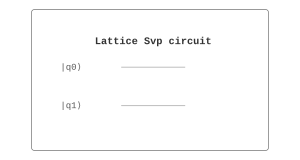
\includegraphics[width=0.6\textwidth]{../../images/lattice_svp_circuit.svg}
\end{center}

\subsection{数学推导}

格最短向量问题：
\begin{equation}
\min_{v \in L \setminus \{0\}} \|v\|
\end{equation}

其中 $L$ 是格，$v$ 是格向量。

\textbf{量子算法}：
\begin{enumerate}
  \item 将格编码为量子态
  \item 用 QFT 提取格结构
  \item 用振幅放大找到最短向量
\end{enumerate}

\subsection{几何解释}

格最短向量问题在格空间中寻找最短向量。量子叠加允许同时探索所有格向量。

\section{代码详解}

\begin{verbatim}
from quonic.algorithms import lattice_svp

# lattice_svp(basis, n_qubits)
# basis: 格基
# n_qubits: 量子比特数

result = lattice_svp(
    basis=[[1, 0], [0, 1]],
    n_qubits=4
)

# result.vector: 最短向量
# result.length: 最短长度
# result.circuit: 量子电路
print(f'Shortest vector: {result.vector}')
print(f'Length: {result.length}')
\end{verbatim}

\section{进阶用法}

\subsection{场景 1：不同格}

\begin{verbatim}
from quonic.algorithms import lattice_svp

# 不同格
basis1 = [[1, 0], [0, 1]]  # 整数格
basis2 = [[2, 1], [1, 2]]  # 非正交格
basis3 = [[1, 1, 0], [0, 1, 1], [1, 0, 1]]  # 3D 格

for basis in [basis1, basis2, basis3]:
    result = lattice_svp(basis)
    print(f'Shortest vector: {result.vector}')
\end{verbatim}

\subsection{场景 2：高维格}

\begin{verbatim}
from quonic.algorithms import lattice_svp
import numpy as np

# 高维格
n = 4
basis = np.random.randint(0, 10, (n, n)).tolist()
result = lattice_svp(basis, n_qubits=8)
print(f'Shortest vector: {result.vector}')
\end{verbatim}

\subsection{场景 3：格基约化}

\begin{verbatim}
from quonic.algorithms import lattice_svp

# 格基约化
basis = [[2, 1], [1, 2]]
result = lattice_svp(basis, reduce=True)
print(f'Reduced basis: {result.reduced_basis}')
print(f'Shortest vector: {result.vector}')
\end{verbatim}

\section{适用场景}

\subsection{密码学}

格最短向量问题是格密码学的基础。格密码学是后量子密码学的重要分支。

\subsection{后量子密码学}

格最短向量问题的量子可解性推动了后量子密码学的发展。NIST 已经标准化了基于格的加密算法（如 CRYSTALS-Kyber）。

\subsection{格基约化}

格最短向量问题可以用于格基约化。格基约化是格密码学中的重要工具。

\section{常见问题}

\subsection{格最短向量问题和大数分解有什么关系？}

格最短向量问题是格密码学的基础，大数分解是 RSA 密码学的基础。两者都是密码学中的困难问题。

\subsection{量子计算机能破解格密码学吗？}

量子计算机可以在多项式时间内求解近似格最短向量问题，但精确求解仍然是困难的。格密码学被认为是对量子计算机安全的。

\section{学习路径}

\subsection{前置知识}
\begin{itemize}
  \item 格理论
  \item 量子傅里叶变换
  \item 振幅放大
\end{itemize}

\subsection{继续学习}
\begin{itemize}
  \item 后量子密码学
  \item 格基约化
  \item 格密码学
\end{itemize}

\section{完整示例代码}

\subsection{示例 1：基本格最短向量问题}

\begin{verbatim}
from quonic.algorithms import lattice_svp

basis = [[1, 0], [0, 1]]
result = lattice_svp(basis)
print(f'Shortest vector: {result.vector}')
\end{verbatim}

\section{下载}

\begin{itemize}
  \item [lattice\_svp.py](https://github.com/ChrisLee0721/QuoNic/blob/main/examples/lattice_svp/lattice_svp.py)
\end{itemize}

\end{document}
